\documentclass{acm_proc_article-sp}

\usepackage[usenames, dvipsnames]{color}
\usepackage{times}
\usepackage{xspace}
\usepackage{textcomp}
\usepackage{wrapfig}
\usepackage{graphicx}
\usepackage{url}
\usepackage{amsmath, amssymb}
\usepackage[protrusion=true,expansion=true]{microtype}
\usepackage{comment}
\usepackage{alltt}
\usepackage{appendix}
%\usepackage{algorithm}
%\usepackage{algorithmic}
\usepackage{booktabs}

%\linespread{0.975}

%\pdfinfo{/Title (Computation and Controlled Coincidence in Dedalus)}

\usepackage{txfonts}
%\newcommand{\DT}{\mathcal{T}}
%\newcommand{\DS}{\mathcal{S}}
\newcommand{\DT}{T}
\newcommand{\DS}{S}
\newcommand{\Consts}{\mathcal{C}}
\newcommand{\Vars}{\mathcal{A}}
%\newcommand{\pos}{\protect{$_{pos}$}}
%\newcommand{\nega}{\protect{$_{neg}$}}
% RCS: Would like to use the above ones, but can't get them to work in Dedalus env.
\newcommand{\pos}{\_pos}
\newcommand{\nega}{\_neg}

\newcommand{\jmh}[1]{{\textcolor{red}{#1 -- jmh}}}
\newcommand{\paa}[1]{{\textcolor{blue}{#1 -- paa}}}
\newcommand{\rcs}[1]{{\textcolor{green}{#1 -- rcs}}}
\newcommand{\nrc}[1]{{\textcolor{magenta}{#1 -- nrc}}}
\newcommand{\wrm}[1]{{\color{BurntOrange}{#1 -- wrm}}}
\newcommand{\smallurl}[1]{{\small \url{#1}}}

\newtheorem{example}{Example}
\newtheorem{definition}{Definition}
\newtheorem{lemma}{Lemma}
\newtheorem{observation}{Observation}

%\def\slang{synchronous Dedalus\xspace}
\def\lang{\textsc{Dedalus}\xspace}
\def\slang{\textsc{Dedalus\ensuremath{_{{0}}}}\xspace}
%\def\synclang{{Dedalus\ensuremath{_{\large 0}}}\xspace}
\newcommand{\naive}      {na\"{\i}ve\xspace}
\newcommand{\Naive}      {Na\"{\i}ve\xspace}
%dedalus environment for code

\newenvironment{Dedalus}{
\vspace{0.5em}\begin{minipage}{0.95\textwidth}%\linespread{1.3}
\begin{alltt}\fontsize{9pt}{9pt}\selectfont}
{\end{alltt}\end{minipage}\vspace{0.5em}}

\newcommand{\dedalus}[1]{\texttt{\fontsize{9pt}{9pt}\selectfont #1}}

\begin{document}

\title{Consistency Analysis in Bloom: A Logical Approach}
\numberofauthors{4}

\author{
\alignauthor
Peter Alvaro
\alignauthor
Neil Conway
\alignauthor
Joseph M. Hellerstein
\and
\alignauthor
William R. Marczak
}

%\conferenceinfo{POPL '11}{Austin, TX, USA} 
%\copyrightyear{2011} 
%\copyrightdata{[to be supplied]}

%\title{Computation and Controlled Coincidence in Dedalus} 
%%Format\titlenote{(Produces the permission block, copyright information and page numbering). For use with ACM\_PROC\_ARTICLE-SP.CLS V2.6SP. Supported by ACM.}}
%
% You need the command \numberofauthors to handle the "boxing"
% and alignment of the authors under the title, and to add
% a section for authors number 4 through n.

%\numberofauthors{4}

%\authorinfo{Peter Alvaro$^\ast$ \quad William R. Marczak$^\ast$ \quad Neil
%Conway$^\ast$ \quad Joseph M. Hellerstein$^\ast$ \\ \quad David Maier$^\dagger$
%\quad Russell Sears$^\ddagger$ \quad Rastislav Bod\'{i}k$^\ast$}
%{$^\ast$University of California, Berkeley \quad $^\dagger$Portland State University \quad $^\ddagger$Yahoo! Research}
%{\{paa, wrm, nrc, hellerstein, bodik\}@cs.berkeley.edu \quad maier@cs.pdx.edu \quad sears@yahoo-inc.com}
% \authorinfo{William R. Marczak}
%            {University of California, Berkeley}
%            {wrm@cs.berkeley.edu}
% \authorinfo{Neil Conway}
%            {University of California, Berkeley}
%            {nrc@cs.berkeley.edu}
% \authorinfo{Joseph M. Hellerstein}
%            {University of California, Berkeley}
%            {hellerstein@cs.berkeley.edu}
%\authorinfo{David Maier}
%           {Portland State University}
%           {maier@cs.pdx.edu}
%\authorinfo{Russell Sears}
%           {Yahoo! Research}\emph{}
%           {sears@yahoo-inc.com}
% \authorinfo{Rastislav Bodik}
%            {University of California, Berkeley}
%            {bodik@cs.berkeley.edu}
\maketitle

\begin{abstract} 
\jmh{I excised the POPL abstract that was pasted here.  I think we need a clean slate.  The last paragraph of the intro is probably close to what we want.}
\end{abstract}

\section{Introduction}
%Our research is motivated by two hard problems in distributed systems.  First,
\wrm{show examples of the problems (not necessarily code) -- evolving state and unreliable communication}

%Distributing any system introduces nondeterminism.  For example, one may
%distribute a computation over many inexpensive, but unreliable, commodity
%machines (e.g. RAID).  The status of internet links and widely distributed
%nodes is inherently more unreliable than multiple cores on a single die, or
%multiple CPUs in a single computer.  

%We present {\bf \lang}, a foundation language for programming and
%reasoning about distributed systems.  

%We correct deficiencies in earlier attempts, and introduce a compelling notion
%of non-determinism in the language.  We specifically use non-determinism to
%reason about {\em when} a deduction becomes visible, including the possibility
%that the deduction will never be visible.  Programmers can constrain this
%non-determinism by using well-studied techniques in distributed systems, such as
%Lamport Clocks 


Traditional database systems are based on declarative query languages that
specify transformations as dataflows over an updatable store.  Such query
languages are either not expressive enough to capture common programming
constructs \wrm{like what?}, or are at best awkward to use in this fashion.
\wrm{todo: transition that explains Datalog's birth from these languages... I
don't know enough to write it} The family of logic-based database languages, of
which Datalog is the progenitor, represent expressive programming languages
that produce similar dataflow representations.  Datalog is purely deductive: a
program specifies the rules by which the derived relations are populated based
on a static database, which is never updated.  Recent programming language
research has explored the use of Datalog-based languages for expressing
distributed systems.  Because the state of any complex system evolves with its
execution, these efforts were forced to extend the Datalog model by admitting
updates, additions and deletions of the EDB.  Unfortunately, these previous
attempts were plagued with ambiguities about how and when state changes occur
and become visible, putting a heavy burden on the programmer to ensure even
simple properties, such as atomicity of updates over time.

In contrast to reasoning about state change procdurally, \lang observes
that this concept is intuitively expressed as invariants over {\em time}.  In
this work, we present a formal model of Datalog augmented with time extensions.
By reifying time as data an introducing it into the logic, \lang eliminates
previous ambiguities, ensures atomicity of updates and makes it possible to
express system invariants that can guarantee liveness properties, a key
challenge in building distributed systems.

\section{Consistency and Logical \\ Monotonicity (CALM)}
In this section we present a strong connection between distributed consistency and logical monotonicity.  This discussion informs the language and analysis tools we develop in subsequent sections.

A key problem in distributed programming is reasoning about consistency in the face of {\em
temporal nondeterminism}: the delay and re-ordering of messages and data across
nodes.  Because delays can be unbounded, analysis typically focuses on ``eventual consistency'' after all messages have been delivered~\cite{vogels}.  A sufficient condition for eventual consistency is {\em order independence}: the independence of program execution from temporal
nondeterminism.

% \jmh{We need to pivot to a discussion of monotonicity and logic programming.  Trick: motivate declarative languages via disorderliness?  May be better to be more direct.}
% Programming models based on sets are attractive in this regard, because they keep programmers from making assumptions about the order of data arrival.  \nrc{Next sentence is confusing/vague to me.} But unordered inputs alone are not sufficient: there is still a question of handling delays as set contents stream (or stall) across a network. 
Order independence is a key attribute of declarative languages based on sets, which has led most notably to the success of parallel databases.  But even set-oriented languages can require a degree of ordering in their execution if they are sufficiently expressive.
The theory of relational databases and logic programming provides a framework to reason about these issues. \emph{Monotonic} programs---e.g., programs expressible via selection, projection and join---can be implemented by streaming algorithms that incrementally produce output elements as they receive input elements; the final order or contents of the input will never cause any earlier output to be ``revoked'' once it has been generated.\footnote{Formally, in a monotonic logic program any true statement continues to be true as new axioms---including new facts---are added to the program.}   
\emph{Non-monotonic} programs---e.g., those that contain aggregation or anti-join operations---can only be implemented correctly via blocking algorithms that do not produce any output until they have received all tuples in logical partitions of an input set. 
%%\nrc{The meaning of ``complete logical subset'' in the preceding sentence is unclear.} \jmh{switched to ``logical set partitions'', which is at least technically well-defined, though perhaps makes for vague english.  The example right after hopefully clears this up, no?}  
For example, aggregation queries need to receive entire ``groups'' before producing aggregates, which in general requires receiving the entire input set.

The implications for distributed programming and delayed messaging are clear. Monotonic programs are easy to distribute: they can be implemented via streaming set-based algorithms that produce actionable outputs to consumers while tolerating message reordering and delay from producers.  By contrast, even simple non-monotonic tasks like counting are difficult in distributed systems.  As a mnemonic, we say that \emph{counting requires waiting} in a distributed system: in general, a complete count of distributed data must wait for all its inputs, including stragglers, before producing the correct output.
% ; the alternative is to risk generating outputs that may be prove to be inconsistent with the full input once it arrives.    For example, an antijoin may output a row incorrectly if it does not wait for all the input records; similarly a SUM may be incorrectly reported as below a threshhold if only a subset of the records are summed.  

``Waiting'' is specified in a program via \emph{coordination logic}: code that (a) computes and transmits auxiliary information from producers to enable the recipient to determine when a set has completely arrived across the network, and (b) postpones production of results for consumers until after that determination is made.  Typical coordination mechanisms include sequence numbers, counters, and consensus protocols like Paxos or Two-Phase Commit.
% Our language, \emph{Bud}, omits coordination logic
% from non-monotonic operators by default, and forces the user to specify it.
% This is because badly-designed coordination logic can be a performance penalty,
% and this seems like a hard problem for an optimizer to approximate (an exact
% solution is undecidable).  In any case, this is the hard component of
% distributed systems programming, so a language should focus programmer effort
% on it.  
%Monotonic operators require no coordination logic.

Interestingly, these coordination mechanisms themselves typically involve counting.  For example, Paxos requires message counting to establish that a majority of the members have agreed to a proposal; Two-Phase Commit requires message counting to establish  that all members have agreed.  Hence we also say that \emph{waiting requires counting}, the converse of our earlier mnemonic.  

Our observations about waiting and counting illustrate the crux of what we call the \emph{CALM} principle: the tight relationship between Consistency And Logical Monotonicity.  Monotonic programs \emph{guarantee} eventual consistency under any interleaving of delivery and computation.  By contrast, non-monotonicity---the property that adding an element to an input set may revoke a previously-valid element of an output set---requires coordination schemes that ``wait'' until inputs can be guaranteed to be complete.  

Obviously we wish to minimize the use of coordination, because of well-known
concerns about latency and availability in the face of message delays during
coordination.  We can use the CALM principle to develop checks for distributed
consistency in logic languages, where conservative tests for monotonicity are
well understood. A simple syntactic check is often sufficient: if the program
does not contain any of the symbols in the language that correspond to
non-monotonic operators (e.g., \texttt{NOT IN} or aggregate symbols), then it is
monotonic and can be implemented without coordination, regardless of any
read-write dependencies in the code.  These conservative checks can be refined
further to consider semantics of predicates in the language. For example, the
expression ``\texttt{MIN(x) $< 100$}'' is monotonic despite containing an aggregate, by
virtue of the semantics of \texttt{MIN} and $<$: once a subset $S$ satisfies this
test, any superset of $S$ will also satisfy it.  Further refinements along
these lines exist, increasing the ability of program analyses to verify
monotonicity.
%More advanced whole-program analyses can take into account whether possibly
%non-monotonic conclusions can ever be consistent with other checks in the
%program; while undecidable in general, conservative tests with constraint
%propagation are often possible.  
% 
% It may also be useful to understand which portions of the program's execution
% or output may be affected by network non-determinism, and which are
% deterministic.  In this case, a static or runtime analysis could perform
% \emph{taint tracking} of network nondeterminism.  %Intuitively, a tuple is
% tainted if it is the transitive result of some %non-monotonic operator.

In cases where an analysis cannot guarantee monotonicity of a whole program, it can instead provide a conservative assessment of the points in the program where coordination may be required to ensure consistency.  For example, a shallow syntactic analysis could flag all non-monotonic predicates in a program (e.g., \texttt{NOT IN} tests or predicates with aggregate values as input).
We call the loci suggested by this analysis the program's \emph{points of
order}. A program with non-monotonicity can be made consistent by including coordination logic at its points of order.  

The reader may observe that because ``waiting requires counting,'' adding coordination logic actually increases the number of points of order in a program since it is non-monotonic.  To avoid this problem, the coordination logic must be hand-verified for consistency, after which annotations on the coordination logic can inform the analysis tool to (a) skip the coordination logic in its analysis, and (b) skip the point of order that the coordination logic handles.  

Because analyses based on the CALM principle operate with information about program semantics, they can avoid coordination logic in cases where traditional read/write analysis would require it.  Perhaps more importantly, as we will see in the next sections, logic languages and the analysis of points of order can help programmers redesign code to achieve goals of minimizing coordination.

%%\jmh{Should we say this: in the full paper, we will more directly show how CALM analysis relates to read/write analyses like serializability?}

% 
% In the general case, it is undecidable to verify whether they have done this
% correctly.  In fact, the introduction of coordination logic may involve
% additional non-monotonic operators (for example, two-phase commit has a
% non-monotonic "COUNT users = COUNT messages" statement).  There are a variety
% of possible solutions to this problem.  One option is for expert programmers
% (i.e. us) to encapsulate a suite of coordination protocols in a library, and
% manually verify the correctness of each protocol.  Another option is to develop
% various static analyses in the style of stratification tests for Datalog.
% \wrm{not sure how we can introduce additional detail here without pulling in
% tons of knowledge dependencies} 

% \wrm{addressed this} \jmh{At minimum, we should assert formal proof in one
% direction: purely Monotonic deduction can be done without coordination.  Start
% with explaining syntactic montonicity, perhaps via SQL, Datalog and MapReduce.
% Then enrich this by saying that single-node non-monotonicity is OK (if it's
% acyclic).} \wrm{i don't think it's okay if it's acyclic -- it's only okay if it
% does not depend on any network messages}  \jmh{  We should then enrich further
% by introducing the non-syntactic, ``instance-oriented'''' style monotonicity:
% saying that individual monotonic deductions---i.e. any monotonic tuple
% lineage---can be computed without coordination.  Give intuitive examples that
% are database instance-dependent (a la local stratification), and that are
% program-semantics dependent (a la universal constraint stratification).  The
% latter should do escrow transactions, and/or tee up shopping cart.}

% \wrm{addressed this} \jmh{Now you can talk at least in casual terms about a
% check for consistency: check the program for non-monotonicity.  Can probably do
% intuition of the data dependency here, and hint at how we'll do taint tracking
% later.}

% \wrm{not sure if this is true, also not sure what "universal-constraint-style
% analyses" you are referring to} \jmh{Now that we've said that ``counting
% requires waiting'', point out that ``waiting requires counting'': coordination
% protocols are basically threshhold tests on distributed count aggregates.
% Hence any check for consistency like the one above will flag the coordination
% logic as a problem.  Our solution: either expert programmers (us) verify the
% modules, or we develop universal-constraint-style analyses to validate them.}

% \wrm{i think we decided the other direction of CALM was false.  consider
% committed choice.  that's non-monotonic any way you look at it (except for the
% definition I tried to sell you durig the POPL submission that we ultimately
% rejected, because we believed monotonic should mean "has a monotonic
% representation in FOL")} \jmh{Finally, introduce the Bi-directional CALM
% Conjecture: that non-monotonic deduction (at the individual tuple level)
% requires coordination.  We can wave hands here about this requiring a crisper
% definition of coordination than we needed before.}

% \wrm{not sure what this means} \jmh{Occurs to me there's a disconnect here with
% the intro---in the intro we said that programming without coordination relates
% to ``loose'' consistency.  We should show a case where for the
% universal-constraint scenario, a read-write consistency analysis would flag
% this as bad, and a transaction manager would forbid it.}

\section{Adding Lattices to Bloom}
\label{sec:lang}

In this section, we introduce \lang, an extension of Bloom that allows monotonic
programs to be written using arbitrary lattices. We begin by reviewing the
algebraic properties of lattices, monotone functions, and morphisms. We then
introduce the basic concepts of \lang and detail the builtin lattices provided
by the language. We also show how users can define their own lattice types using
a simple Ruby API.

% is this the right place for this?
When designing \lang, we decided to extend Bloom to include support for
lattices rather than building a new language from scratch. Hence, \lang is
backward compatible with Bloom and was implemented with relatively minor
changes to the Bud runtime. This design decision also required that we consider
rules written over lattices should interoperate with rules that use traditional
Bloom relations; we added several \lang features to ease this interoperability,
which we describe in Section~\ref{sec:bloom-interop}.

\subsection{Definitions}
\label{sec:lattice-defn}
A \emph{bounded join semilattice} is a triple $\langle S, \lor, \bot\rangle$,
where $S$ is a poset, $\lor$ is a binary operator (called ``join'' or ``least
upper bound''), and $\bot \in S$. $\lor$ is associative, commutative, and
idempotent. For all $x, y \in S$, $x \lor y = z$, where $x \leq_S z, y \leq_S
z$, and there is no $z' \in S$ such that $z' <_S z$ (where $<_S$ is the partial
order associated with the poset $S$). Note that although the underlying set only
has a partial order, the least upper bound is defined for all elements $x,y \in
S$. The distinguished element $\bot$ is the smallest element in $S$; this
implies that $x \lor \bot = x$ for all $x \in S$. For brevity, we use the term
``lattice'' to mean ``bounded join semilattice'' in the rest of this paper.

% XXX: note that algebraic properties that must be satisfied by morphisms and
% monotone functions
A \emph{monotone function} from poset $S$ to poset $T$ is a function $g: S \to
T$ such that $\forall a,b \in S: a \leq_S b \Rightarrow g(a) \leq_T g(b)$. That
is, $g$ maps elements of $S$ to elements of $T$ in a manner that is consistent
with the partial orders of both posets.

% XXX: mention that morphisms must be distributive with respect to the lub of
% their domain, whereas monotone functions don't need to be?
A \emph{morphism} from lattice $\langle X, \lor_X, \bot_X\rangle$ to lattice
$\langle Y, \lor_Y, \bot_Y\rangle$ is a function $f$ such that, $\forall a,b \in
X: f(a \lor_X b) = f(a) \lor_Y f(b)$. That is, $f$ allows elements of $X$ to be
converted into elements of $Y$ in a way that preserves the lattice properties.
Note that all morphisms are monotone functions but the converse is not true in
general.

\subsection{Language concepts}
In \lang, state is represented using lattices and computation is expressed as
functions over lattices. A lattice in \lang is analogous to a collection type in
Bloom, while a lattice element corresponds to a particular collection value. For
example, the \texttt{lset} lattice provides similar functionality to the
set-oriented collections provided by Bloom; an element of the \texttt{lset}
lattice is a particular set value. In the terminology of object-oriented
programming, a lattice is a class that obeys a certain interface and an element
of a lattice is an instance of that class.

As in Bloom, the lattices used by a \lang program are declared in a
\texttt{state} block. More precisely, the declarations in the state block
introduce identifiers that are associated with lattice elements; over time, the
binding between identifiers and lattice elements is updated to reflect state
changes in the program. For example, line~\ref{line:quorum-lset-decl} of
Figure~\ref{fig:lattice-quorum} declares an identifier \texttt{votes} that is
mapped to an element of the \texttt{lset} lattice. As more votes are received,
the lattice element associated with the \texttt{votes} identifier
changes---specifically, it moves upward in the \texttt{lset} lattice.

\subsubsection{Computation in \lang}
Statements take the same form in both Bloom and \lang. The identifier on the lhs
of a statement can refer to either a set-oriented collection or a lattice. The
expression on the rhs can contain both traditional relational operators (applied
to Bloom collections) and method invocations (applied to lattice elements).

Note that if the lhs of a statement refers to a lattice, the statement's
operator must be either \verb|<=| or \verb|<+|, denoting instaneous or deferred
deduction. \lang does not currently support a notion of ``deletion'' for
lattices. Lattices do not directly support asynchronous communication (via the
\verb|<~| operator), but lattice elements can be embedded into channels (as
described in Section~\ref{sec:bloom-interop}).

\subsection{Builtin lattice types}
\label{sec:lattice-builtins}

\begin{table*}[t]
\begin{tabular}{|l|l|l|l|l|}
\hline
\textbf{Name} & \textbf{Description} & \textbf{Merge} & \textbf{Morphisms} &
\textbf{Monotone functions}\\
\hline
\texttt{lbool} & Boolean lattice (false $\to$ true) & & \texttt{when\_true} & \\
\texttt{lmax} & Max over an ordered domain & &\texttt{gt},
\texttt{gt\_eq}, \texttt{+}, \texttt{-} & \\
\texttt{lmin} & Min over an ordered domain & &\texttt{lt}, \texttt{lt\_eq},
\texttt{+}, \texttt{-} & \\
\texttt{lset} & Set of values & & \texttt{intersect}, \texttt{product},
\texttt{project} & \texttt{size} \\
\texttt{lpset} & Set of non-negative numbers & &
\texttt{intersect}, \texttt{product}, \texttt{project}& \texttt{size}, \texttt{sum} \\
\texttt{lbag} & Multiset of values & & \texttt{intersect},
\texttt{project}, \texttt{mult(k)}, \texttt{+} & \texttt{size}\\
\texttt{lmap} & Map from key to lattice values & &
\texttt{intersect}, \texttt{project}, \texttt{at(k)}, \texttt{key?(k)} & \texttt{size}\\
\hline
\end{tabular}
\caption{The builtin lattices in \lang.}
\label{tbl:builtin-lattices}
\end{table*}

Table~\ref{tbl:builtin-lattices} lists the builtin lattices provided by
\lang. Many common distributed protocols can be expressed using these lattices
(e.g., the causal delivery protocol described in Section~\ref{sec:causal}).

Note that \emph{size} is a monotone function provided by several lattices, but
it is not a morphism. This is because \texttt{size} cannot be distributed over
the merge functions of those lattices. For example, \ldots

\subsection{Lattice API}
\label{sec:lattice-api}
In \lang, each lattice has an associated Ruby class, which we call the
\emph{lattice class}. An instance of this class is called a \emph{lattice
  element}. A lattice element represents a single point in the lattice---i.e., an
element of the poset associated with the lattice.

A lattice class is a normal Ruby class that meets a certain API contract. Every
lattice class inherit from the builtin \texttt{Bud::Lattice} class, and
must also define two methods:
\begin{itemize}
\item \texttt{initialize(i)}: given a Ruby object \emph{i}, this method
  constructs a new lattice element that ``wraps'' \emph{i} (\texttt{initialize}
  is just the normal Ruby syntax for defining a constructor). By convention, the
  Ruby value wrapped by a lattice element is assigned to a Ruby member variable
  \texttt{@v}. If $i$ is the null reference, this method returns the least
  element of the lattice.

\item \texttt{merge(e)}: given a lattice element \emph{e}, this method returns the
  lattice element that is the least upper bound of $\{e, \textit{self}\}$. This method must
  satisfy the algebraic properties summarized in Section~\ref{sec:lattice-defn}---in
  particular, it must be commutative, associative, and idempotent. Note that
  \emph{e} must have the same class as \emph{self}.
\end{itemize}
Lattice elements are \emph{immutable} (e.g., \texttt{merge} functions should
construct a new lattice element rather than modifying one of their inputs
in-place). Efficient lattice implementations may \emph{share structure} on merge
operations, as is common practice for immutable data structures in functional
programming languages~\cite{Okasaki1999}. % XXX: maybe not the right place for this

\begin{figure}[t]
\begin{scriptsize}
\begin{lstlisting}
class Bud::SetLattice < Bud::Lattice
  wrapper_name :lset

  def initialize(x=[])
    # Reject invalid input (elided)
    @v = x.uniq # Remove duplicates from input
  end

  def merge(i)
    self.class.new(@v | i.reveal)
  end

  morph :intersect do |i|
    self.class.new(@v & i.reveal)
  end

  morph :pro do |&blk|
    @v.map(&blk)
  end

  ord_map :size do
    Bud::MaxLattice.new(@v.size)
  end
end
\end{lstlisting}
\end{scriptsize}
\caption{The implementation of the \texttt{lset} lattice in Ruby.}
\label{fig:lattice-set}
\end{figure}

\subsection{Integration with set-oriented logic}
\label{sec:bloom-interop}

\begin{figure}[t]
\begin{scriptsize}
\begin{lstlisting}
class ShortestPaths
  include Bud

  state do
    table :link, [:from, :to, :c]
    table :path, [:from, :to, :next_hop] => [:c]
    table :min_cost, [:from, :to] => [:c]
  end

  bloom do
    path <= link {|l| [l.from, l.to, l.to, MinLattice.new(l.c)]}
    path <= (link*path).pairs(:to => :from) do |l,p|
      [l.from, p.to, l.to, p.c + l.c]
    end
    min_cost <= path {|p| [p.from, p.to, p.c]}
  end
end
\end{lstlisting}
\end{scriptsize}
\caption{A \lang program to compute the all-pairs shortest paths of a
  graph.}
\label{fig:lattice-spaths}
\end{figure}

\lang provides two features to ease integration of lattice-based code with
traditional Bloom programs that manipulate set-oriented collections.

\subsubsection{Implicit fold}
% XXX: this ignores the fact that Bloom collections consist of sets of tuples,
% whereas implicit fold works for sets of singleton values
% XXX: refer to shortest paths program as practical example
This feature enables set-oriented collections to be more easily used as input to
lattices. If a \lang statement has a set-oriented collection on the rhs and a lattice
on the lhs, the lattice merge function is used to ``fold over'' the elements of
the collection. That is, each element of the collection is converted to a
lattice element (via the appropriate lattice constructor); then the set of
lattice elements are merged together (via repeated application of the
\texttt{merge} method). In our experience, this is typically the behavior
intended by the user.

\subsubsection{Collections with embedded lattice values}
It would be convenient to allow lattice elements to be stored as attributes of
tuples that appear in set-oriented Bloom collections. Furthermore, Bloom
provides several facilities (e.g., network communication, persistent storage,
module interfaces) as collections with special semantics; it would be
unfortunate if a redundant set of facilities would be necessary to support
lattice-based code. A simple solution would be to extract the underlying Ruby
value from the lattice element (e.g., using the \texttt{reveal} method), and
then store that value as a tuple attribute in a set-oriented
collection. Unfortunately, that would introduce needless non-monotonicity into
the program.

Storing lattice elements as attributes of tuples in set-oriented collections
introduces several challenges. Consider a simple \lang statement that derives tuples
with a lattice element as an attribute value:
\begin{verbatim}
    t1 <= t2 {|t| [t.x, lat_foo]}
\end{verbatim}
where \texttt{t1} and \texttt{t2} are Bloom relations and \texttt{lat\_foo}
identifies a lattice; suppose that the first column of \texttt{t1} is the
relation's key. The value associated with \texttt{lat\_foo} can change over the
course of the fixpoint computation (specifically, it can grow ``upward''
according to the lattice's partial order, as more values are merged into the
lattice). Implemented naively, this might result in multiple \texttt{t1} tuples
with different values for the second attribute, which would violate
\texttt{t1}'s key (the first column of \texttt{t1} would not functionally
determine a single value for the second column).

This problem could be avoided by placing constraints on the evaluation order of
statements: for example, we could require that all potential changes to
\texttt{lat\_foo} be completed before rules that embed \texttt{lat\_foo} could
be evaluated. This would effectively stratify the program according to lattice
embedding rules, which would disallow cycles through lattice
embeddings~\cite{Apt1988}. This would reject intuitively reasonable programs; it
also seems unsatisfying to require stratification of monotonic programs.

% Clarify this
Instead, \lang allows rules to produce multiple tuples that differ only in their
embedded lattice values. During the course of the fixpoint computation, those
values are merged together using the appropriate lattice merge function. This is
safe because Bud stratifies programs according to non-monotonic operators;
hence, any operators that might be applied to an embedded lattice value before
it has been determined exactly must be monotonic. Nevertheless, this solution is
somewhat counterintuitive because tuples in Datalog relations are traditionally
immutable: once a fact is known to be true, its value remains the
same.% \footnote{Bloom facts can be deleted, but this is an explicit non-monotonic
  % operation that can only occur between timesteps. Conceptually, Bloom models
  % update as the retraction of the previous version of a fact and the insertion
  % of a new fact~\cite{dedalus}.}
% Should we note that we might add an option to disable this behavior for
% particular attributes, or explain more about why this might be considered
% weird?

For similar reasons, we currently disallow lattice values from being used as
keys in Bloom collections. It might be possible to relax this restriction in
certain ``safe'' cases, but we have not found this limitation to be problematic
to date.

\subsection{Confluence in \lang}
\nrc{TODO: justify that CALM continues to hold for monotonic programs over
  lattices.}

\section{Case Study: Key-Value Store}
\label{sec:kvs}
In this section, we present two variants of a key-value store (KVS) implemented
using Bloom. We begin with an abstract protocol that any key-value store will
satisfy, and then provide both single-node and replicated implementations of
this protocol. We then introduce a graphical visualization of the dataflow in a
Bloom program, and use this visualization to reason about the \emph{points of
  order} in our programs: places in the program where additional coordination
may be required to guarantee consistent results (Section~\ref{sec:calm}).

\subsection{Abstract Key-Value Store Protocol}

\begin{figure}[t]
\begin{scriptsize}
\begin{lstlisting}
module KVSProtocol
  def state
    interface input, :kvput, 
      ['client', 'key', 'reqid'], ['value']
    interface input, :kvget, ['reqid'], ['key']
    interface output, :kvget_response, 
      ['reqid'], ['key', 'value']
  end
end
\end{lstlisting}
\centering
\vspace{-10pt}
\caption{Abstract key-value store protocol.}
\label{fig:kvs-proto}
\end{scriptsize}
\vspace{-2pt}
\end{figure}

Figure~\ref{fig:kvs-proto} specifies a protocol for interacting with an abstract
key-value store. The protocol comprises two input interfaces (representing
attempts to insert and fetch items from the store) and a single output interface
(which represents the outcome of a fetch operation). To use an implementation of
this protocol, a Bloom program can store key-value pairs by inserting facts into
\texttt{kvput}. To retrieve the value associated with a key, the client program
inserts a fact into \texttt{kvget} and then looks for the corresponding response
tuple in \texttt{kvget\_response}. In both cases, the client program must supply
a unique request identifier (\texttt{reqid}) to differentiate tuples in the
event of multiple concurrent requests.

A module which uses a key-value store but is indifferent to the specifics of the
implementation may simply mix in this protocol specification and postpone
committing to a particular implementation until runtime. As we will see shortly,
an implementation of the KVSProtocol is a collection of Bud rules that read
tuples from the protocol's input interfaces and send results to the output
interface.

\subsection{Single-Node Key-Value Store}
\label{sec:simple-kvs}
\begin{figure}[t]
\begin{scriptsize}
\begin{lstlisting}
module BasicKVS
  include KVSProtocol

  def state
    table :kvstate, ['key'], ['value'] (*\label{line:kvs-state}*)
  end

  declare
  def do_put
    kvstate <+ kvput.map{|p| [p.key, p.value]} (*\label{line:kvs-put}*)
    jst = join [kvstate, kvput], [kvstate.key, kvput.key] (*\label{line:kvs-join}*)
    kvstate <- jst.map{|b, p| b} (*\label{line:kvs-clean}*)
  end

  declare
  def do_get
    getj = join [kvget, kvstate], [kvget.key, kvstate.key] (*\label{line:kvs-getjoin}*)
    kvget_response <= getj.map do |g, t|
      [g.reqid, t.key, t.value]
    end
  end
end
\end{lstlisting}
\centering
%%\includegraphics[width=0.55\linewidth]{fig/basickvs.pdf}
\vspace{-10pt}
\caption{Single-node key-value store implementation.}
\label{fig:kvs-impl}
\end{scriptsize}
\vspace{-2pt}
\end{figure}

Figure~\ref{fig:kvs-impl} contains a simple single-node implementation of the
abstract key-value store protocol. Key-value pairs are stored in a persistent
table called \texttt{kvstate} (line~\ref{line:kvs-state}). When a \texttt{kvput}
tuple appears, its key-value pair is stored in \texttt{kvstate} at the immediately
following timestep (line~\ref{line:kvs-put}).  If the given key already exists in
\texttt{kvstate}, we want to replace the key's old value. This is done by
joining \texttt{kvput} against the current version of \texttt{kvstate}
(line~\ref{line:kvs-join}). If a matching tuple is found, the old key-value pair
is removed from \texttt{kvstate} at the beginning of the next timestep
(line~\ref{line:kvs-clean}). Note that we also insert the new key-value pair
into \texttt{kvstate} in the next timestep (line~\ref{line:kvs-put});
hence, we implement an overwriting update as an atomic deletion and insertion.

\subsection{Replicated Key-Value Store}
\label{sec:rep-kvs}

\begin{figure}[t]
\begin{scriptsize}
\begin{lstlisting}
module ReplicatedKVS
  include BasicKVS
  include MulticastProtocol

  def state
    interface input, :kvput, (*\label{line:rep-put-beg}*)
      ['client', 'key', 'reqid'], ['value']  (*\label{line:rep-put-end}*)
  end

  declare
  def replicate
    send_mcast <= kvput.map do |k| (*\label{line:send-mcast-beg}*)
      unless members.include? [k.client]  (*\label{line:not-rep}*)
        [k.reqid, [@addy, k.key, k.reqid, k.value]]   (*\label{line:marshall}*)            
      end
    end (*\label{line:send-mcast-end}*)
  end

  declare
  def apply_put
    kvput <= mcast_done.map{|m| m.payload}  (*\label{line:mcast-done}*)

    kvput <= pipe_chan.map do |d| (*\label{line:mcast-peer-beg}*)
      if d.payload.fetch(1) != @addy
        d.payload
      end
    end (*\label{line:mcast-peer-end}*)
  end
end
\end{lstlisting}
\vspace{-10pt}
\caption{Replicated key-value store implementation.}
\label{fig:kvs-repl}
\end{scriptsize}
\vspace{-2pt}
\end{figure}

Next, we extend the basic key-value store implementation to support replication
(Figure~\ref{fig:kvs-repl}). To communicate between replicas, we use a simple
multicast library implemented in Bloom; the complete source code for this
library can be found in Appendix~\ref{app:network-code}. To send a multicast, a
Bloom program inserts a fact into \texttt{send\_mcast}; a corresponding fact
appears in \texttt{mcast\_done} when the multicast has completed.\footnote{XXX:
  error handling.} The multicast library also provides the membership of the
multicast group in a table called \texttt{members}.

Our replicated key-value store is implemented on top of the single-node
key-value store described in the previous section. When a new key is inserted by
a client, we multicast the insertion to the other replicas
(lines~\ref{line:send-mcast-beg}--\ref{line:send-mcast-end}). To avoid repeated
multicasts of the same inserted key, we avoid multicasting updates we receive
from another replica (line~\ref{line:not-rep}). We apply an update to our local
\texttt{kvstate} table in two cases: (1) if a multicast succeeds at the node
that originated it (line~\ref{line:mcast-done}) (2) whenever a multicast is
received by a peer replica
(lines~\ref{line:mcast-peer-beg}--\ref{line:mcast-peer-end}).

Note that the implementation of ReplicatedKVS wants to ``intercept''
\texttt{kvput} events from clients, and only apply them to the underlying
BasicKVS module when certain conditions are met. To achieve this, we
``override'' the declaration of the \texttt{kvput} input interface
(lines~\ref{line:rep-put-beg}--\ref{line:rep-put-end}). In ReplicatedKVS,
references to \texttt{kvput} appearing in the LHS of rules are resolved to the
\texttt{kvput} provided by BasicKVS, while references in the RHS of rules
resolve to the local \texttt{kvput}.  Note that this is unambiguous, because a
module cannot insert into its own input or read from its own output
interfaces. Nevertheless, the current syntax for achieving this is somewhat
cryptic; it might be improved by the addition of a namespace-like concept.

\subsection{Predicate Dependency Graphs}
\begin{figure}[t]
\centering
\includegraphics[width=0.9\linewidth]{fig/mittalk_legend.pdf}
\vspace{-10pt}
\caption{Visual analysis legend. \jmh{Check on the $+/-$ label in the figure.  Is that right, do we ever use $-$?}}
\label{fig:analysis-legend}
\vspace{-2pt}
\end{figure}

Now that we have introduced two concrete implementations of the abstract
key-value store protocol, we now turn to analyzing the properties of these
programs. First, we introduce the graphical dataflow representation used by our
analysis; we then discuss the dataflow graphs generated for the key-value store
programs in the following section.

A Bloom program may be viewed as a dataflow graph with external input interfaces
as sources, external output interfaces as sinks, collections as internal nodes,
and rules as edges. This graph represents the dependencies between the
collections in a program, and can be generated automatically by the Bud
interpreter. A list of the different symbols and annotations in the graphical
visualization can be found in Figure~\ref{fig:analysis-legend}; we provide a
brief summary below.

Each node in the graph is either a collection or a cluster of collections;
tables are shown as rectangles, ephemeral collections (scratch, periodic and
channel) are depicted as ovals, and clusters (described below) as octagons. A
directed edge from node $A$ to node $B$ indicates that $B$ appears in the lhs of
a Bloom rule with $A$ referenced directly, or through a join expression, in the
rhs.  An edge is annotated based on the operator symbol in the rule. If the rule
uses the \texttt{$<$+} or \texttt{$<$-} operators, the edge is marked with
$+$. This indicates that facts traversing the edge ``spend'' a timestep to move
from the rhs to the lhs. Similarly, if the rule uses the \texttt{$<\sim$}
operator, the edge is a dashed line---this indicates that facts from the rhs
appear at the lhs at a non-deterministic future time. If the rule involves a
non-monotonic operation (aggregation, anti-join, or the \texttt{$<$-} operator),
then the edge is marked with a small circle.  To make the visualizations more
readable, any strongly connected component marked with both a circle and a $+$
edge is collapsed into an octagonal ``temporal cluster,'' which can be viewed
abstractly as a single, non-monotonic node in the dataflow. \emph{Points of
  order} are indicated in the graph by an edge with a white circle.  Any
non-monotonic edge in the graph is a point of order, as are all edges incident
to a temporal cluster, including any self-edges.

\subsection{Analysis}
Figure~\ref{fig:pdg-kvs-proto-analysis} presents a visual representation of the
abstract key-value store protocol. The diagram depicts the semantics implied by
the protocol's interfaces: data is inserted into the input interfaces
(\texttt{kvput} and \texttt{kvget}), and results eventually appear in the output
interface (\texttt{kvget\_response}). Naturally, the abstract protocol does not
specify a connection between the input and output events; this is indicated in
the diagram by the red diamond, which denotes an underspecified program. A
concrete realization of the key-value store protocol must, at minimum, supply a
dataflow that connects an input interface to the output interface.

Figure~\ref{fig:pdg-kvs-analysis} shows the visual analysis of the basic KVS
implementation, which supplies a concrete dataflow for the unspecified component
in the previous graph.  \texttt{kvstate} and \texttt{jst} are collapsed into a
red octagon because they are part of a strongly connected component in the graph
with both negative and temporal edges.  Any data flowing from \texttt{kvput} to
the sink must cross at least one non-monotonic point of order (at ingress to the
octagon) and possible an arbitrary number of them (via the octagon's self-edge),
and any path from \texttt{kvget} to the sink must join state potentially
affected by non-monotonicity (because \texttt{kvstate} is used to derive
\texttt{kvget\_response}).

Reviewing the code in Figure~\ref{fig:kvs-impl}, we see that this is
unavoidable.  The contents of \texttt{kvstate} at a given time are defined (in
part; line~\ref{line:kvs-clean}) in terms of its contents at the immediate
previous state and the current input.  Hence the state of \texttt{kvstate} at
any point in time may depend on the order of arrival of \texttt{kvput} tuples.
% We challenge the reader to implement the KeyValueProto interface in a way that
% has no such point of order.



\begin{figure}[t]
\centering
\includegraphics[width=0.4\linewidth]{fig/kvs_proto_pdg.pdf}
\vspace{-10pt}
\caption{Visualization of the abstract key-value store protocol.}
\label{fig:pdg-kvs-proto-analysis}
\vspace{-2pt}
\end{figure}

\begin{figure}[t]
\centering
\includegraphics[width=0.5\linewidth]{fig/basickvs.pdf}
\vspace{-10pt}
\caption{Visualization of the single-node key-value store.}
\label{fig:pdg-kvs-analysis}
\vspace{-2pt}
\end{figure}

\section{Case Study}
\label{sec:case}

\wrm{Re-do case studies in Bud} \wrm{Break cart development down into
iterations} \wrm{How does the language naturally lead us to an order
independent style?  Talk about inserting all sorts of exotic stuff like queues
if we want a highly order-dependent imperative style.}



\section{Experiments}
\label{sec:expr}
We have prototyped our language, execution model, and some of our
optimizations as modifications to the \Pitu system. Our
prototype takes as input \Dlog programs, performs rule localization, and generates a dataflow graph
consisting of \Pitu \xspace{\em elements}. Each element is a node in the dataflow
graph, and performs tasks such as queuing, network processing and
traditional relational operations like joins and aggregations.

The generated execution plan is structurally similar to
Figure~\ref{Dataflow1}, where there are rule strands comprising
chains of elements. Each rule strand takes as input a queue,
corresponding to new tuples for each strand. Our current
implementation uses the PSN algorithm at the tuple granularity. A
new tuple is dequeued and processed by the rule strand to generate new
tuples which are then enqueued at the same node or sent as a network
message for further processing at another node.

Beyond validating our language and implementation, the main goal of our evaluation
is to verify the effectiveness of several of the proposed
optimizations. In evaluating our system, the main metrics that we use
are: 

\vspace{1pt}
\noindent {\bf Convergence time: }The time taken for the query execution
to generate all the query results.

\vspace{1pt}
\noindent {\bf Communication overhead: }The number of bytes transferred
  for each query. We consider both aggregate communication overhead (MB), as well as
  per-node bandwidth (kBps).


In summary, we find:
  
\begin{CompactEnumerate}
\item The aggregate selections optimization reduces communication overhead. Using {\em
  periodic aggregate selections} reduces this overhead further. 

\item The use of magic sets and predicate reordering reduces communication overhead when only a limited number of paths
  are queried. 

\item Multi-query sharing techniques such as query result caching and
  opportunistic result caching demonstrate the potential to reduce communication
  overhead when there are several concurrent queries.

\item On a network with bursty updates, incremental query evaluation
  techniques can recompute paths at a fraction of the cost of
  recomputing the queries from scratch.
  
\end{CompactEnumerate}

%In practice,
%  we have scaled \Sys on up to a thousand processes running on a single
%  machine without any network emulation.} 

\subsection{Setup}

Our experiments are conducted by running our modified \Pitu on 100 nodes
on the Emulab~\cite{emulab}
testbed. This testbed emulates realistic latency and bandwidth constraints seen on the Internet,
  yet provides repeatable experiments under a controlled environment. As input to the Emulab testbed, we use transit-stub
topologies generated using GT-ITM~\cite{gtitm}, a package that is widely used to model
Internet topologies. Our topology has four transit nodes, eight nodes
per stub and three stubs per transit node. Latency between transit nodes
  is $50$ ms, latency between transit nodes and their stub nodes is $10$
ms, and latency between any two nodes in the same stub is $2$
ms. The link capacity is set to $10$ Mbps.

We construct an overlay network over the base GT-ITM topology where
each node is assigned to one of the stub nodes. Each overlay node runs
\Sys on one Emulab machine, and picks four randomly selected
neighbors. Each node has four link tuples, one for each neighbor. Each
link tuple has metrics that include latency (based on the underlying GT-ITM
topology), reliability (link loss correlated with latency),
and a randomly generated value.  

We base our workload primarily on routing
protocols~\cite{declareRoute}, and benchmark four variants of the
same {\em shortest-path} query, differing in the link metric each
seeks to minimize. On all our graphs, we label these queries by their
link metric: {\em Hop-Count}, {\em Latency}, {\em Reliability} and
{\em Random}, respectively. Note that {\em Random} serves as our
stress case: we expect it to have the worst performance among all
queries, because aggregate selections are less
likely to be effective when the aggregate metric is uncorrelated with
the network latency, which determines tuple arrival order during query
execution.
%. These queries are used to compute the optimal paths between all pairs
%  of nodes based on various link metrics. 




%  to less effective aggregate selections. When completed, each of these
%  queries would compute the optimal paths for the {\em fewest
%    hop-count}, {\em lowest aggregate latency}, {\em most
%  reliable} and {\em lowest aggregate random}.  


\subsection{Aggregate Selections}
\label{subsec:expr:aggsel}


\begin{figure}[ht]
\centering
 \begin{minipage}{.45\linewidth}
  \begin{center}
    \epsfig{file=graphs/baseline/bw.ps,width=1.18in,angle=-90}
    \small{\caption{\label{baseline-bw}\emph{\small Per-node Bandwidth (kBps).}}}
    \end{center}
 \end{minipage}
\hfill
 \begin{minipage}{.45\linewidth}
  \begin{center}
    \epsfig{file=graphs/baseline/results.ps,width=1.18in,angle=-90}
    \small{\caption{\label{baseline-convergence}\emph{\small
    Query results over time (seconds).}}}
  \end{center}
 \end{minipage}
\end{figure}

We first investigate the effectiveness of aggregate selections for
different queries. Figure~\ref{baseline-bw} shows the per-node
bandwidth usage against time for the four
queries. Figure~\ref{baseline-convergence} shows the percentage of
eventual best paths completed against time. Our results show that {\em
Hop-Count} converges the most quickly in $4.4$ seconds, followed by
{\em Latency} and {\em Reliability} in $4.9$ seconds and $4.8$ seconds
respectively. {\em Random} has the worst convergence time
of $5.8$ seconds.

During query execution, the communication overhead incurred by all
four queries shows a similar trend
(Figure~\ref{baseline-bw}). Initially, the communication overhead
increases as more and more paths (of increasing length) are derived. After
it peaks at around $19 kBps$ per-node, the communication overhead
decreases, as fewer and fewer optimal paths are left to be derived. In
terms of aggregate communication overhead, {\em Random} incurs the
most overhead ($4.1$ MB), while {\em Hop-Count}, {\em Latency} and
{\em Reliability} use $2.6$ MB, $3.1$ MB and $3.2$ MB,
respectively. The relatively poor performance of {\em Random} is due
to the lack of correlation between the metric and network latency,
leading to a greater tendency for out-of-order arrival of path tuples
that results in less effective use of aggregate selections.


%\subsubsection{Periodic Aggregate Selections}

\begin{figure}[ht]
\centering
 \begin{minipage}{.45\linewidth}
  \begin{center}
    \epsfig{file=graphs/dynamic/bw-3.ps,width=1.18in,angle=-90}
    \small{\caption{\label{periodic-bw}\emph{\small Per-node Bandwidth (kBps).}}}
    \end{center}
 \end{minipage}
\hfill
 \begin{minipage}{.45\linewidth}
  \begin{center}
    \epsfig{file=graphs/dynamic/results-3.ps,width=1.18in,angle=-90}
    \small{\caption{\label{periodic-convergence}\emph{\small
    Query results over Time (seconds).}}}
  \end{center}
 \end{minipage}
\end{figure}

The results in Figures~\ref{periodic-bw} and
\ref{periodic-convergence} illustrate the effectiveness of 
the {\em periodic aggregate selections} approach, as described in
Section~\ref{subsec:aggregateSelections}.  In particular, this
approach reduces the bandwidth usage of {\em Hop-Count}, {\em
Latency}, {\em Reliability} and {\em Random} by $17$\%, $12$\%, $16$\%
and $29$\%, respectively. {\em Random} not only shows the greatest
reduction in communication overhead, its convergence time also reduces from $5.8$
seconds to $5$ seconds. 
%In all experiments we use a wait period of 300
%ms.

%This demonstrate the effectiveness of performing aggregate
%  selections in batches, by buffering up tuples before computing the
%  optimal paths to be sent to neighboring nodes.

\subsection{Magic Sets and Predicate Reordering}
\label{subsec:expr:caching}

\begin{figure}[ht]
\centering
 \begin{minipage}{.45\linewidth}
  \begin{center}
    \epsfig{file=graphs/magiccache/queryBW_random100.ps,width=1.18in,angle=-90}
    \small{\caption{\label{ms-bw}\emph{\small Aggregate communication overhead (MB) with and
    without magic sets and caching}.}}
    \end{center}
 \end{minipage}
\hfill
 \begin{minipage}{.45\linewidth}
  \begin{center}
    \epsfig{file=graphs/correlate/bw-corrshare3.ps,width=1.18in,angle=-90}
    \small{\caption{\label{opportunistic-bw300}\emph{\small
    Per-node Bandwidth (kBps) for message sharing (300 ms delay).}}}
  \end{center}
 \end{minipage}
%\hfill
% \begin{minipage}{.3\linewidth}
%  \begin{center}
%    \epsfig{file=graphs/correlate/bw-corrshare0.05.ps,width=1.5in,angle=-90}
%    \small{\caption{\label{opportunistic-bw50}\emph{\small Per-node Bandwidth (kBps) for
%    correlated sharing (50 ms delay)}}}
%    \end{center}
% \end{minipage}
\end{figure}

Next, we study the effectiveness of combining the use of magic sets
and predicate reordering for lowering communication overhead when the
queries are constrained by randomly chosen sources and
destinations. Our workload consists of queries that request
source-to-destination paths based on the {\em Hop-Count} metric. For
each query, we execute the {\em magic-shortest-path} query
(Section~\ref{sec:magic}). 

Figure~\ref{ms-bw} shows the aggregate communication overhead as the number of
queries increases.  The {\em No-MS} line represents our baseline, and
shows the communication overhead in the absence of rewrites (this
essentially reduces to computing all-pairs least-hop-count). The {\em
MS} line shows the communication overhead when running the optimized
query with no sharing across queries. When there are few queries, the
communication overhead of {\em MS} is significantly lower than that of
{\em NO-MS}. As the number of queries increases, the communication
overhead of {\em MS} increases linearly, exceeding {\em No-MS} after
$170$ queries.

%\subsubsection{Magic Sets with Caching}
%\label{subsec:expr:magic}

In addition, Figure~\ref{ms-bw} also illustrates the effectiveness of
caching (Section~\ref{subsec:multiQuerySharing}). The {\em MSC} line
shows the aggregate communication overhead for magic sets with caching. For
fewer than $170$ queries, there is some overhead associated with
caching. This is due to false positive cache hits, where a cache
result does not contribute to computing shortest paths. However, as
the number of queries increases, the overall cache hit rate improves,
resulting in a dramatic reduction of bandwidth. 
When limiting the choice of destination nodes to $30$\% ({\em
MSC-30\%}) and $10$\% ({\em MSC-10\%}), the communication overhead
levels of at $1.8$ MB, and $1$ MB, respectively. The smaller the set
of requested destinations, the higher the cache hit rate, and
the greater the opportunity for sharing across different queries.
These results are consistent with the results obtained by Loo
\textit{et~al.}~\cite{declareRoute} in a similar experiment,
using the PIER~\cite{pierCidr} simulator.


\subsection{Opportunistic Message Sharing}
\label{subsec:expr:correlated}

We study the impact of performing opportunistic message sharing across
concurrent queries that have some correlation in the messages being
sent. Figure~\ref{opportunistic-bw300} shows per-node bandwidth
usage for running the queries on different metrics
concurrently. To facilitate sharing, we delay each outbound tuple by
$300$ms in anticipation of possible sharing opportunities. The {\em
Latency}, {\em Reliability} and {\em Random} lines show the bandwidth
usage of each query individually. The {\em No-Share} line shows
the total aggregate bandwidth of these three queries without
sharing. The {\em Share} line shows the aggregate bandwidth
usage with sharing. Our results clearly demonstrate the
potential effectiveness of message sharing, which reduces the peak of
the per-node communication overhead from 27 kBps to 16 kBps, and the
total communication overhead by 34\%.

%We repeat the experiment with a lower outbound delay of $50$ ms, and
% observed that there is less sharing achievable across queries. The peak
% per-node bandwidth usage attained with sharing is 22 kBps, which
% is only marginally lower compared to no sharing. The aggregate
% bandwidth usage is reduced by 18\%, which is far less than when the delay is $300$ ms. This clearly
% demonstrates the usefulness in delaying outbound tuples in
% order to facilitate sharing. Determining the correct period at
% runtime based on the query workload is an interesting area for further exploration.

\subsection{Incremental Query Evaluation}
\label{subsec:expr:dynamic}

\begin{figure}[ht]
\centering
 \begin{minipage}{.45\linewidth}
  \begin{center}
    \epsfig{file=graphs/dynamic/bw-random-burb-10.ps,width=1.18in,angle=-90}
    \small{\caption{\label{bursty-bw1}\emph{\small Per-node Bandwidth (kBps) for
    periodic link updates on latency metric (10s update interval).}}}
    \end{center}
 \end{minipage}
\hfill
 \begin{minipage}{.45\linewidth}
  \begin{center}
    \epsfig{file=graphs/dynamic/bw-latency-burb-random-vary.ps,width=1.18in,angle=-90}
    \small{\caption{\label{bursty-bw2}\emph{\small
    Per-node Bandwidth (kBps) for periodic link updates (interleaving 2s and 8s
    update interval).}}}
  \end{center}
 \end{minipage}
\end{figure}


In our final experiment, we examine the overhead of incrementally
maintaining query results in a dynamic network. We run the queries
over a period of time, and subject the network to burst updates as
described in Section~\ref{sec:dynamic}.  Each update burst involves
randomly selecting 10\% of all links, and then updating the cost
metric by up to 10\%. We use the shortest-path random metric since it
is the most demanding in terms of bandwidth usage and
convergence time.

Figure~\ref{bursty-bw1} plots the per-node communication overhead,
when applying a batch of updates every $10$ seconds. Two points are worth
noting. First, the time it takes the query to converge after a burst
of updates is well within the $5$ second convergence time of running the
query from scratch (Figure~\ref{periodic-convergence}). This is
reflected in the communication overhead, which increases sharply after
a burst of updates is applied, but then disappears long before the next
burst of updates (Figure~\ref{bursty-bw1}). Second, each burst peaks
at $6 kBps$, which is only 32\% of the peak bandwidth and 26\% of the
aggregate bandwidth of the original computation. Our results clearly
demonstrate the usefulness of performing incremental query evaluation
in response to changes in the network, as opposed to recomputing the
queries from scratch.     

We repeat our experiment on a more demanding update workload
(Figure~\ref{bursty-bw2}), where we interleave update intervals that
are $2$ seconds and $8$ seconds, the former interval being less than
the from-scratch convergence time of $5$ seconds. We observe that
despite the fact that bursts are sometimes occurring faster than
queries can run, bandwidth usage is similar to the less
demanding update workload. When the update interval is $2$ seconds, we
notice periods of sustained bandwidth usage, however the peak
usage remains at $6$ kBps as before.
%When the interval is subsequently increased to $8$ seconds, the query computation
%quiesces as shown by the reduction of bandwidth usage to $0$ kBps. 




 
%At the same
% time, there is also no noticeable improvement to the convergence
% time relative to the previous experimental setup, as the extra messages
% negate any impact of lowering the periodic interval. Figuring out the
% correct interval at runtime base on parameters such as opportunities for sharing, allowing for
% out-of-sync queries issued at different times to ``catch-up and
% share'', and adapting based on the rate of change in the
% network are interesting aspects of adaptive query processing for further exploration.


%\subsubsection{Hybrid Rewrites}
%\label{subsec:expr:hybrid}

%TO FILL IN. 

%Compare bandwidth and convergence with all-pairs shortest path
%computation (Figure~\ref{zone-bw}).

%Compare with flood-based source routing and show that this is cheaper in
%bandwidth (Figure~\ref{zone-route}). 


%\subsection{Summary}
%Summarize the key points in evaluation.



%\subsubsection{Gossip-based Approximations}
%\label{subsec:expr:hybrid}

%OPTIONAL if time permits.

%Graph for gossip:

%\begin{itemize}
%\item Y-axis: Bandwidth / Path length
%\item X-axis: Time
%\end{itemize}

%Repeat for different gossip rate (\% of paths not propagated to neighbors). Show
%tradeoffs of path quality and bandwidth. 





%\subsection{Query Approximations}
%\label{subsec:expr:queryApprox}

%\begin{itemize}
%\item Y-axis: Convergence / Bandwidth 
%\item X-axis: Time 
%\end{itemize}

%Demonstrate bandwidth reduction vs loss of results quality. Show CDF of
%computed path costs for approximation and without approximation.


%\subsection{Multi-Objective Queries}
%\label{subsec:expr:multiObj}

%Optional. Show highly correlated (latency, loss-rate) multi-objective
%can result in savings. 


% LocalWords:  dataflow PSN kBps bursty Emulab ITM Mbps bw MSC Loo al

\section{Conclusion}
\label{sec:conclusion}
And thus, we conclude.

%\scriptsize
%\begin{spacing}{0.9}
\bibliographystyle{abbrv}
\bibliography{cidr11,declarativity}
%\end{spacing}

%%\appendix
%%\section{Proof of Lemma 1}
\begin{proof}
%First, we prove an isomorphism between stable models, and finite prefixes of stable models.  Scan a stable model of a program timestamp by timestamp.  
We first present an algorithm for computing ultimate models, and argue that the algorithm computes exactly the stable models of the \lang program.  We then argue this algorithm can be run on our operational formalism, show how operational traces correspond with prefixes of stable models.

Any \lang program without asynchronous rules is a $\text{Datalog}_1S$ program, and the algorithm given in~\cite{tdd} computes an ultimate model in polynomial space\footnote{The class of {\em multi-seperable}~\cite{tdd-poly} \lang rules, which comprises all \lang programs $P$ with guarded asynchrony and persisted EDB, and their coordinations $\textsc{Coord}(P)$, can be executed in polynomial time.} in the size of the input.  The algorithm evalutes the program for $2^G + e$ consecutive timesteps, where $G$ is the number of instantiations of the non-temporal attributes of the program rules, using all combinations of constants in the Herbrand Universe, and $e$ is the maximum timestamp of any EDB fact.  At each step, the algorithm updates information on observed periodicities of facts.  When the algorithm terminates, any fact with a periodicity of 1 is regarded as part of the ultimate model.

For asynchronous rules, the natural distributed analog of the algorithm above simultaneously executes one instance for each node \dedalus{n}, using values of $G$ and $e$ computed from $E_{\text{\dedalus{{\scriptsize n}}}}$.  Each instance has its own local clock, which intuitively corresponds to the timestamp attribute in the model-theoretic semantics.  Nodes communicates over channels with arbitrary delay and message re-ordering.  When another node \dedalus{m} derives a fact at \dedalus{n}, it encloses its local clock value, \dedalus{t}; \dedalus{n} must consider this fact until time \dedalus{t}, in the style of Lamport Clocks.  Note that this behavior is implied by the model-theoretic semantics---remote asynchronous rules state that their deductions are visible at the destination at a time later than the body temporal attribute at the source.  Further, note that Lamport Clocks only introduce the constraint that if message $a$ ``happens before'' $b$, in other words $a$ directly or transitively causes $b$ to be sent, then $T(a) < T(b)$.  If $a$ and $b$ are concurrent, there is some execution where $T(a) \geq T(b)$.

When \dedalus{n} processes a received message, the number of constants available to \dedalus{n} may increase, and thus a node's $G$ may increase to $G'$.  Furthermore, the node may need to execute over this new fact for $2^{G'}$ additional timesteps.  If only finitely many messages are sent, this algorithm requires polynomial space.  In the case that infinitely many messages are sent, we only need to process each message $2^{G'}$ times: the maximum period of any fact is $2^{G'}$, as every incoming fact needs to have a chance (in some execution) to join with any deduction, at any time during its period, with which it is ``concurrent''.  Keeping track of the number of times we have seen each fact also requires polynomial space.  When the algorithm is done running for $2^{G'}$ steps, it pauses, waiting for new network input that it has not seen enough times.  If all nodes are paused and no outstanding messages exist, then the collection of all period 1 facts at all instances of the algorithm comprises an ultimate model.

We claim that the algorithm can generate every ultimate model---every message has the opportunity to join with another concurrent message or its transitive consequents at any point during their period, and has the opportunity to join with a causally related message during the range of times allowed by the model-theoretic asynchronous constraint (identical to the Lamport Clock condition used in the algorithm).

Note that we can execute this algorithm on our operational formalism.  Evaluating a single timestamp of a \lang program corresponds to the evaluation of a Datalog program, which is a polynomial time computation, and the Turing Machines can also maintain the necessary state about periods and message counts.
%2) Intuitively, the operational model is based on n Turing Machines, one per value of node(), which independently step sequentially through time and communicate via channels with
%non-deterministic delay.  At each timestep t they run a datalog fixpoint computation that evaluates P on ``projection(E_n, t)'' (notation needed); this takes polynomial
%time~\cite{immerman}.  At the end of this fixpoint there are three sets of relevant facts: local, synchronous facts that have timestep t+1 and become part of ``projection(E_n,
%t)'', local asynchronous facts whose timestep is chosen non-deterministically to be greater than t and become part of later timesteps, and remote asynchronous facts.  The
%timestamps in this third class of facts are chosen non-deterministically ``at the receiver'' to model delay, in a way that observes traditional causality
%restrictions~\cite{lamportclocks}.
%3) Any \lang program without  async rules is a Datalog_{1S} program, and the above intuition is captured by the algorithm given in~\cite{}, computing an ultimate model in
%polynomial space in the size of the input.  In the presence of asynchronous rules, this formalize needs to be expanded to account for the asynchronous advancement of time through
%\dedalus{successor} at each node.  The PSPACE guarantees of~\cite{} are not shown to hold for such programs, but in Appendix Foo we show that the following Lemma holds for all
%\lang programs under this model
\end{proof}

\section{Proof of Lemma 2}
\begin{proof}
We begin by assuming that \dedalus{node} contains the identifiers of each of the $n$ nodes.  Since the atemporal fragment of \lang is FO[LFP], we can represent a polynomial-time bounded Turing Machine using only atemporal rules in \lang~\cite{immerman-ptime}.  In addition to normal operations, the Turing Machine can place items into a queue---\cite{dedalus} shows how to model queues in \lang---or send messages to other nodes---modeled by an asynchronous communication rule with \dedalus{queue} in the head.  A node persists the contents of the tape across time if the queue is empty, using a rule like \dedalus{tape(\dbar{X})@next <- tape(\dbar{X}), !queue(\dbar{\_});}.  If the queue is non-empty, the computation skips a timestamp (leaving \dedalus{tape} empty), and then atomically copies the contents of \dedalus{queue} to \dedalus{tape}.  The ultimate model of this program is exactly the final contents of the tape on every node if the computation halts.  Otherwise, the program's ultimate model is empty: \dedalus{tape} facts only exist every other timestamp, and for any Turing Machine predicate \dedalus{r} we can create \dedalus{r'}, and create a mutual recursive cycle to ensure neither \dedalus{r} nor \dedalus{r'} contains facts at every timestamp:

\begin{Dedalus}
r(\dbar{X})@next <- r'(\dbar{X});
r'(\dbar{X})@next <- r(\dbar{X});
\end{Dedalus}

We can play a somewhat similar trick for \dedalus{queue} by having local messages alternate between going into \dedalus{queue} and \dedalus{queue'}.  Thus, no local queue message will be part of the ultimate model.  Remote messages will still go into \dedalus{queue}: this still leaves the case that the exact same message repeatedly arrives at a node at every timestamp forever, by chance.  We can dispense of this case by assuming the channels interconnecting the Turing Machines forbid it.
\end{proof}

\section{Proof of Lemma 3}
\begin{proof}
Our proof proceeds via construction of a two counter machine in \lang, inspired by the construction in~\cite{undecidable-datalog}. We briefly review two counter machines.  A two counter machine's state is captured in the state of its two counters (natural numbers), and in its control state.  A two counter machine has a transition function: $\delta: \Sigma \times \{=, >\} \times \{=, >\} \rightarrow \Sigma \times \{inc, dec\} \times \{inc, dec\}$

$\Sigma$ is a finite set of states (for simplicity we assume a finite subset of the natural numbers), $=$ indicates a counter is equal to zero, and $>$ indicates a counter is greater than zero.  $inc$ and $dec$ indicate that a counter should be incremented, or decremented respectively.

We represent the state of a two counter machine using the \linebreak \dedalus{cnfg(T,S,C1,C2)} relation, where \dedalus{T} represents ``time'' (note this is not the same as the timestamp attribute), \dedalus{S} is the state (in $\Sigma$), and \dedalus{C1} and \dedalus{C2} are the values of the two counters.  In order to support $inc$ and $dec$, we would like to make use of the \dedalus{succ} relation.  However, \lang conventions forbid the use of this infinite relation outside of the timestamp attribute.  Thus, we posit the \dedalus{fin\_succ(X,Y)} EDB relation, which represents a finite prefix of the successor relation.  Since it is EDB, its contents may be arbitrary.  If \dedalus{fin\_succ} is malformed, then the machine's execution may be incorrect.  In particular, our model of the machine may accept an input, whereas the actual machine would not have accepted that input.  We illustrate how to constrain the contents of \dedalus{fin\_succ} below:

\begin{Dedalus}
malformed() <- fin_succ(_,0);
malformed() <- fin_succ(X,Y), fin_succ(X,Z), Y != Z;
malformed() <- fin_succ(Y,X), fin_succ(Z,X), Y != Z;
malformed() <- fin_succ(X,Y), X >= Y;
\end{Dedalus}

For a given EDB, the two counter machine either halts in the accepting state or halts in a non-accepting state.  It cannot run forever since the EDB (in particular, the \dedalus{fin\_succ} relation) is finite.

We construct a \lang program that nondeterministically decides to either run the machine on the input provided (and for the length of \dedalus{fin\_succ} provided, or declare that the machine will never accept without running it.  If the machine ever accepts some input, then we would like this to induce two different ultimate models -- one generated by a trace where we run the machine and it accepts, and one generated by a trace where we decide to not run the machine, and thus we implicitly reject.  We describe the program below. 

Initially, we nondeterministically decide whether to run the machine or not, by sending two messages (0 and 1) to a remote node (\dedalus{decider}).  If both message arrive simultaneously, then the decider responds to run the machine.  Otherwise, the decider responds to declare failure:

%\jmh{should we use a hashmark for constants?  I would say no.}
\begin{Dedalus}
//send two messages to the decider
message(#D, 0)@async <- decider(D);
message(#D, 1)@async <- decider(D);

//decider responds to computer
run_machine(#computer)@async <- message(0),
                                message(1);
declare_failure(#computer)@async <- message(0),
                                    !message(1);
declare_failure(#computer)@async <- !message(0),
                                    message(1);
\end{Dedalus}

Each mapping in the transition function is expressed by a \lang rule with \dedalus{!malformed()} and \dedalus{!declare\_failure()} in its body.  For example, the rule $\delta(3, > =) = (7, inc, dec)$ would be represented as:

\begin{Dedalus}
cnfg(S,7,D1,D2) <- cnfg(T,3,C1,C2), C1 > 0, C2 == 0,
                   fin_suc(T, S), fin_succ(C1, D1),
                   fin_succ(D2, C2), !malformed(),
                   !declare_failure();
\end{Dedalus}

We declare success or failure as follows:

\begin{Dedalus}
reject() <- !accept();
accept() <- cnfg(20,_,_); //20 is the accepting state
accept()@next <- accept();
\end{Dedalus}

If we choose to declare failure, or the machine halts in a non-accepting state, whether it is due to incompleteness or malformedness \dedalus{fin\_succ}, or actual halting, then the ultimate model will contain \dedalus{reject}.  If the machine halts in an accepting state, then the ultimate model will contain \dedalus{accept}.  Thus, if we can decide confluence of this program, then we can decide whether a two-counter machine halts on any input.
\end{proof}


%%\section{attic}

\textbf{stuff we don't want to get rid of but don't know what to do with}

\subsection{Kinds of Relations}
    
%%\jmh{Ack ... deductive rules are unsafe, and technically Datalog-neg forbids them due to the free variable in the head.  So you will need to expand your language to include an acceptable notion of per-timestep safety (as Maier suggested), at which point it's not a subset of Datalog-neg.  Would be nice to be able to say ``\lang is a subset of (Datalog + \{set of addons\})'' but that would require defining the acceptable saftey before defining timestamps (which are a restriction).}
%\nrc{Title is too long: EDB, IDB, and NDB instead?}
In a \lang program, there are three kinds of relations:
extensional, {\em intensional} or {\em nondeterministic}.

%\nrc{We define the term ``extensional predicate'' before, but not
%  ``extensional relation''.}
\begin{definition}
%
An \emph{intensional} relation is a relation that appears
in the head of one or more atemporal or inductive rules in the program, but
never in the head of an asynchronous rule.~\nrc{``atemporal'' rules
  have not been defined.}
%
\end{definition}
\begin{definition}
%
A \emph{nondeterministic} relation is a relation that
appears in the head of one or more asynchronous rules in the program.
%
\end{definition}
We refer to the sets of ground atoms in intensional and nondeterministic
predicates respectively as the IDB, and NDB.

%\jmh{introduction of the MDB doesn't seem useful, actually.  I'd drop this,
%and if you need to define a ``mutable'' relation as one that participates in
%the head of a temporal rule, you can do so as needed.}
The EDB, IDB, and NDB are all pairwise disjoint.  Intuitively, the distinction
between the NDB and IDB is that the NDB is determined nondeterministically~\nrc{clumsy} from
the EDB, IDB and NDB, while the IDB is determined deterministically from the
EDB, IDB and NDB.  Thus, given a \lang instance, all IDB predicates that do
not transitively depend on NDB predicates can be evaluated deterministically.
We will refer to facts, ground atoms in the EDB, and \emph{events}
interchangeably, for reasons which will soon become clear.
%%\jmh{The only reason to worry about the MDB being non-deterministic is @sync, which you didn't in fact need to introduce yet.  Again, I don't see this discussion being useful.}

\subsection{Traces}


\begin{figure}[t]
  \centering
  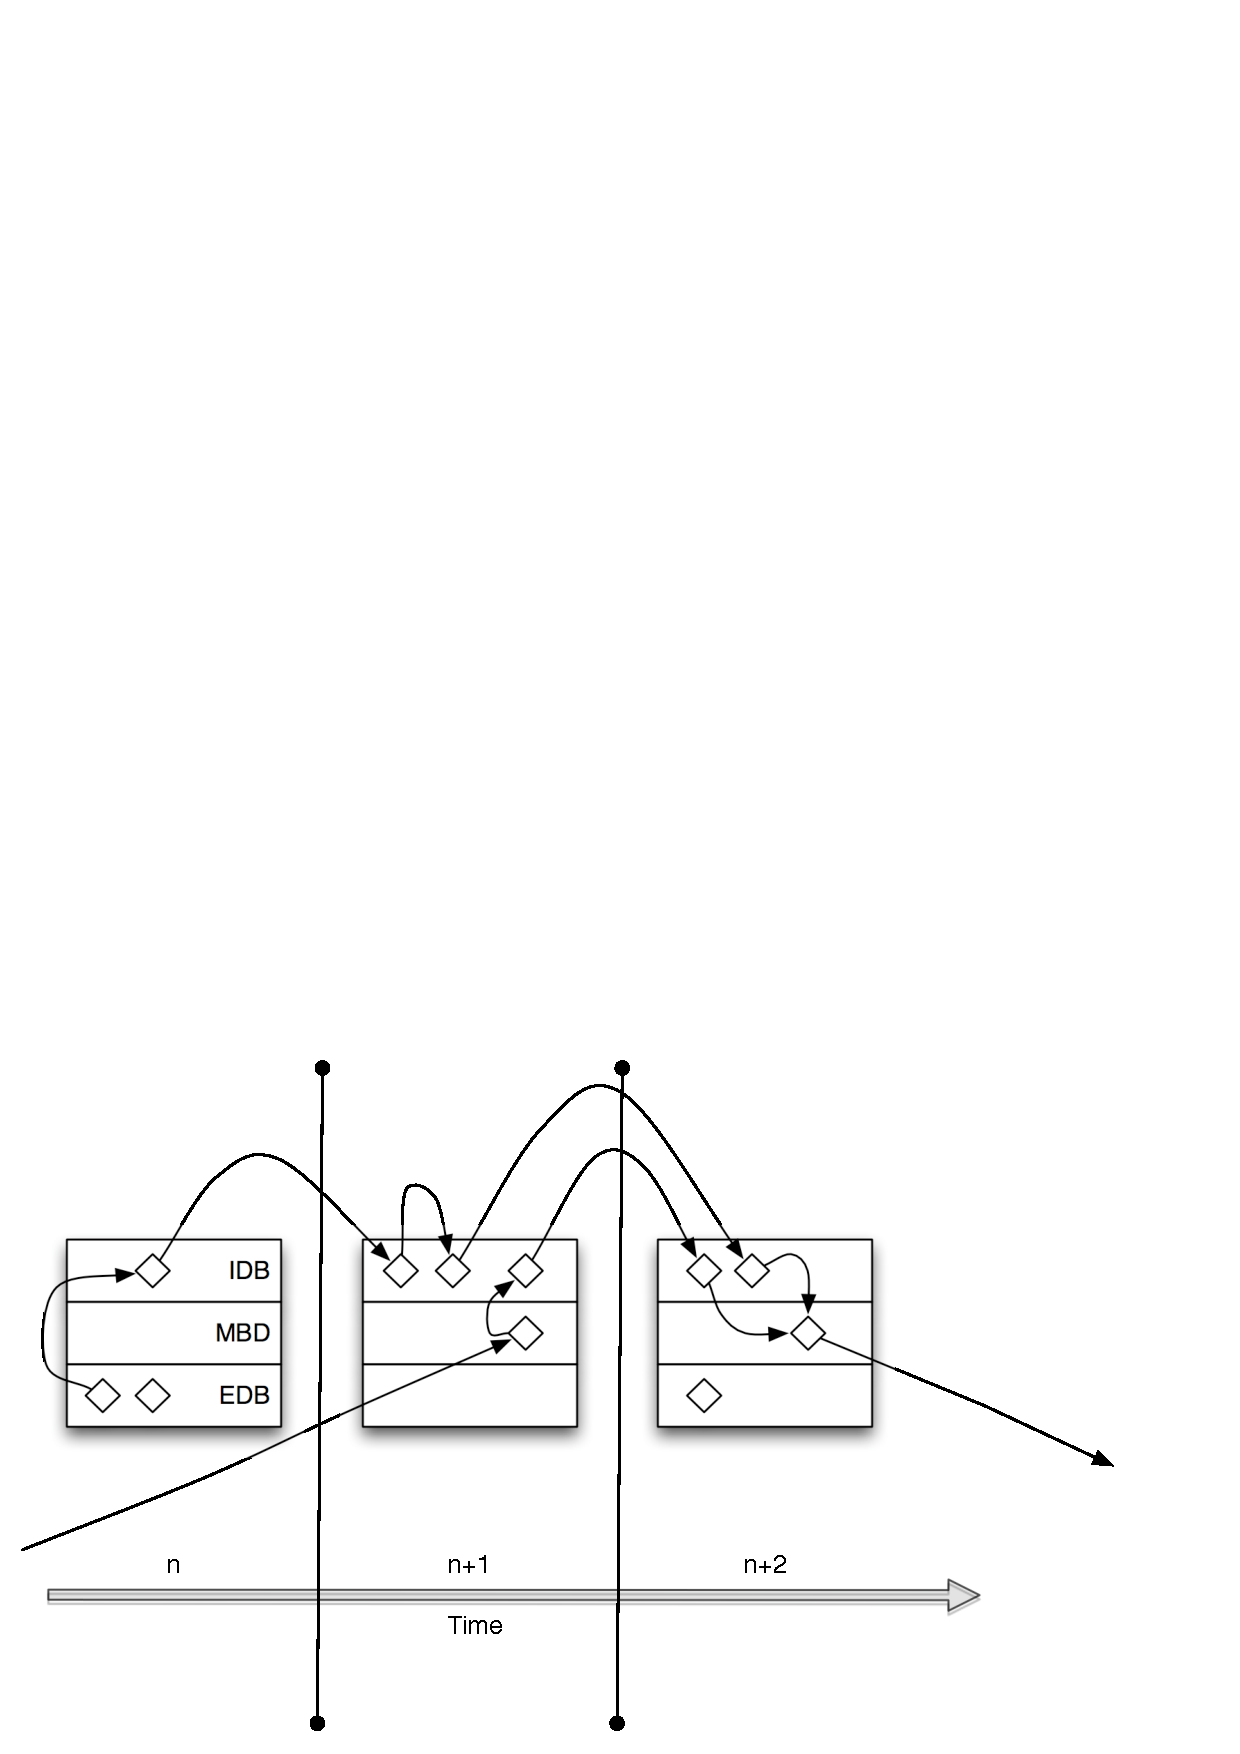
\includegraphics[width=1\linewidth]{figures/edbidbmdb.pdf}
  \label{fig:edbidbmdb}
  \caption{Derivations across time in IDB and MDB relations.}
\vspace{-8pt}
\end{figure}

\paa{this section (its placement \emph{and} content) is somewhat problematic given the current structure
of the draft.  We've established the notion of finite preambles of a (possibly infinite) EDB.  A trace is basically just
an interpretation (a set of ground atoms) -- by calling it a ``trace" we're connoting a post-hoc \wrm{warning: post hoc is undefined} interpretation.
A trace that is just EDB is sufficient, given a program, to augment the trace with IDB and MDB atoms such that
the resulting trace is a model (by simply running a fixpoint computation).  For a program with no async rules, the EDB of input is sufficient to recreate the
program execution exactly -- that is to say, to reproduce the single minimal model of the program given the EDB.
It is \emph{not} sufficient to recreate the execution of a program with async rules: intuitively, we'd need to include in 
the trace the complete MDB, for every entry in it potentially corresponds to one of many possible minimal models.
perhaps we just want to show that there is a method (drop the async rules and run a fixpoint computation to generate
the IDB from MDB and EDB) to regenerate a "complete trace" (ie minimal model) from EDB $\cup$ MDB}

%Consider a non-empty EDB $E$, an empty MBD $M$ and IDB $I$ and a program $P$.  Evaluating $P$ against $E$ may derive facts in $M$ and $I$.

\begin{definition}
A \emph{trace} is any set of facts from the EDB, NDB or IDB of a \lang program evaluation.
\end{definition}

Any trace for a \lang instance $(P,E)$ is an interpretation of $(P,E)$.
%\wrm{lol, why do we need the notion of an incomplete trace?}

\begin{definition}
%
A \emph{complete trace} of an evaluation of a \lang instance is the union of
the given EDB with the derived IDB and MDB.
%
\end{definition}

\begin{lemma}
%
A complete trace of a \lang instance $(P,E)$ is its unique minimal model.
%
\end{lemma}

%\begin{lemma}
%%
%For any bound on $successor$, a complete trace of a \lang  instance $(P,E)$ has a unique minimal model.
%%
%\end{lemma}

If we evaluate E given P, and P is stratifiable, the resulting set of ground atoms is a minimal model.
In our case, however, successor causes our EDB to be infinite, so the minimal model of any \lang program 
with temporal rules is potentially infinite.  \paa{but we'd like to show that a weaker property holds: that for any value $N$
in the \emph{successor} relation, the resulting program has a minimal model.}
\wrm{we either already showed this, or our theorems above are wrong.}


\begin{definition}
A \emph{minimal trace} is a subset of a complete trace that excludes any IDB ground atoms derived through an inductive
rule.
\end{definition}

A minimal trace of a \lang program $P$ is equivalent to the complete trace of which is is a subset -- the latter may be derived from the former by repeated
applications of inductive rules.  However, a given a \lang instance $(P, E)$ and a minimal trace T (where $E \subset T$), a fixpoint
computation will most likely \emph{not} yield a minimal model, because new tuples may be added to the MDB that represent a component 
of a different minimal model, and because these may affect the IDB.  The set of ground atoms $EDB \cup MDB_{old} \cup IDB_{new}$
\emph{may} may be a minimal model, iff $IDB_{new} = IDB_{old}$.  \paa{actually I am not sure if that is true}.  
$(EDB \cup MDB_{old} \cup IDB_{new} \cup IDB_{old})$ is certain to be a model, but is only minimal if $IDB_{new} \subset IDB_{old}$.

A minimal trace records the nondeterminism caused by the delay or reordering of async rules, and
is equivalent to the original program execution.  

\begin{definition}
A \emph{reduced trace} is a minimal trace with normalized time suffixes starting with 0 and increasing by 1 at each step.
\end{definition}

show a (trivial) procedure for reduction and make some claims about equivalences without entanglement.

\begin{definition}
A \emph{event trace} is a \lang EDB.
\end{definition}

An event trace and program P may be used to generate a new IDB and MDB.  The MDB is virtually certain to differ from that of another
execution, while the IDB may differ, depending on its dependency on the MDB.  The union of these three databases is of course a
minimal model, but probably not the same minimal model from another execution.  \paa{but can we say that it will often be true that if we project 
out the time attribute from every predicate, the minimal models will be the same? it won't always be true...}



\subsection{EDB Preambles}

\rcs{I've never seen someone use ``preamble'' to refer to this concept.  Why not call it a prefix?}

A \slang instance's EDB may be arbitrarily large.  In this section we introduce
the notion of a {\em preamble} -- a truncation of the EDB, and prove an
equivalence between full evaluation of a preamble and incremental evaluation
based on evaluation of an earlier preamble.
%A \slang instance may receive arbitrarily many external input tuples over the
%course of its execution, but should not wait arbitrarily long before
%performing deductions.  In this section we introduce the notion of EDB
%preambles, and prove an equivalence between two types of evaluation.

%In general, the EDB of a \slang instance may be infinite, and may lead to unsafe evaluations even when \emph{successor} is derived from it
%as in a post-hoc evaluation.

\begin{definition}
A \emph{preamble} $\alpha_{n}$ of an EDB $\Gamma$ is the set of facts in $\Gamma$ whose timestamp is less than or equal to $n$.
\end{definition}

If the EDB is finite, then it has a maximum timestamp $\top$, \rcs{is successor now part of the EDB? Otherwise, there is no max timestamp} and
$\alpha_{\top}$ = $\Gamma$.  \wrm{I don't think we use $\top$ anywhere else}
Because each preamble is a superset of all preambles with lower indices, we
have the monotonicity property:

$\forall \alpha_{i}, \alpha_{j} \in \Gamma : (i < j) \to (\alpha_{i} \subseteq \alpha_{j})$

%\paa{to your point, bill, I switched the lemma and proof below to one of IDB equivalence in the posthoc vs. continual interpretation
%rather than an inductive proof that every model in the series is minimal.  there is probably a very similar proof of the latter
%that we could include in the next section after introducing minimal models, stratification etc}

\wrm{todo: disuss replacing FP with some derivation tree thing}
\begin{definition}
%
Let $F$ be the set of all finite subsets of possible atoms.  Let $P$ be the set
of all finite subsets of possible rules.  Let $FP : P \times F \mapsto F$ be
the function representing the \emph{fixpoint} computation carried out by a
datalog interpreter.  That is, $FP_p$ takes an EDB to its corresponding IDB.
%
\end{definition}


\begin{lemma}
\label{lem:costmodel}
%
Let $i \in \mathbb{Z}$.  Then, $FP_p(\alpha_{i+1} \cup FP_p(\alpha_i)) =
FP_p(\alpha_{i+1})$.
%
\end{lemma}

%%this could (with some work) lead to an inductive proof
%%that an infinite model is minimal.  we could prove the (weaker?) property that
%%the infinite series of models of increasing finite preambles of an EDB are all 
%%minimal if one of them is.

\begin{proof}

%%Inductive step:

%%if we assume that some program P and finite preamble $\alpha_n$ of a trace $\Gamma$ produce a minimal model, 
%%then it follows that a preamble $\alpha_{n+1}$ and the IDB produced by the previous model produce a minimal model.

by contradiction. Assume $\exists i \in \mathbb{Z}$ such that:
$FP_p(\alpha_{i+1} \cup FP_p(\alpha_i)) \neq FP_p(\alpha_{i+1})$

{\bf Case 1:} $\exists A \in FP_p(\alpha_{i+1} \cup FP_p(\alpha_i)) : A \not\in FP_p(\alpha_{i+1}).$

This implies that $A$ is transitively dependent on atoms in $\alpha_{i+1} \cup
FP_p(\alpha_i)$.  However, if $A$ is transitively dependent only on atoms in
$\alpha_{i+1}$, then $A$ would be in $FP_p(\alpha_{i+1})$.  Thus, $A$ must be
transitively dependent on some atoms in $FP_p(\alpha_{i})$.  But $\alpha_{i}
\subset \alpha_{i+1}$, so this implies that $A$ is transitively dependent on
some atom in $\alpha_{i+1}$, which means $A \in FP_p(\alpha_{i+1})$.  This
contradicts our assumption, thus no such $A$ may exist.

{\bf Case 2:} $\exists A \in FP_p(\alpha_{i+1}) : A \not\in FP_p(\alpha_{i+1} \cup FP_p(\alpha_i)).$

This implies that $A$ is transitively dependent on $\alpha_{i+1}$.  In order
for $A \not\in FP_p(\alpha_{i+1} \cup FP_p(\alpha_i))$, we need $A$ to depend
negatively on an atom $B \in FP_p(\alpha_i)$.  But $B$ transitively depends on
an atom $C \in \alpha_i$.  $C \in \alpha_{i+1}$ by definition (if $B$ is
extensional, then $C=B$), so $B \in FP_p(\alpha_{i+1})$, so $a \not\in
FP_p(\alpha_{i+1})$.  This contradicts our assumption, thus no such $A$ may
exist.
%If $I_2 \neq I_3$, it must be the case that either there exists a ground atom in $I_2$ that is not in $I_3$, or that is in
%$I_3$ and not in $I_2$.  
%Take the former case first.  This means there is an atom $A$ that is entailed by P given $FP(\alpha_{j} \cup FP(\alpha_{i}))$
%but not entailed by P given $\alpha_{j}$, so it must be in $I_1$.   The only circumstances under which an atom in
%$I_1$ would not occur in the IDB $FP(\alpha_{j})$ is if there is a fact $B$ in $\alpha_{j}$ 
%corresponding to a negated subgoal in a rule $r$ in P upon which $A$ depends.  However, for this to occur, because a ground atom 
%in $I_1$ cannot depend upon a ground atom from the ``future", that fact $B$ would need to have occurred at some time less than 
%or equal to the to timestamp of atom $A$.  But this is not possible, because all timestamps in $\alpha_{j}$ that are not in any $\alpha_{k} | k<j$
%are strictly higher than any timestamps in $\alpha_{k}$.  Hence the first case leads to contradiction.
%As for the second case...
\end{proof}

\subsection{Cost Model}
%%\newdef{definition}{Definition}
Lemma~\ref{lem:costmodel} implies that we can trade computation cost for
storage cost in evaluation of a \slang program. 

%In the continuous interpretation of a \slang program, it is in general only
%useful to remember facts at a single timestamp in a predicate.  Two ways to
%approach this issue are to either always persist the ``latest'' version, or
%continuously re-derive the latest version.  These are represented in the naive
%deductive and overwriteable storage implementations below.

%\begin{figure}[t]
%\begin{tabular}{ll} \hline
%%Rule Pattern & Idiom & Prepare & Propose & Election \\ \hline \hline
%$d$ & Cost of a deductive step \\
%$s$ & Cost of storing a tuple \\
%$r$ & Cost of reading a tuple \\ 
%$t$ & Number of tuple derivations from deductive rules \\ 
%\hline
%$S$ & Set of tuples inserted \\
%$U$ & Set of tuples updated \\
%$P$ & Set of stored tuples, with time projected out \\ 
%$T$ & Set of stored tuple timestamps \\ 
%$Q$ & Set of query timestamps \\ \hline 
%\end{tabular}
%\caption{Cost model.}
%\label{fig:breakdown}
%\end{figure}


%\subsubsection{Naive Deductive Implementation}

%To evaluate a trace consisting of $S$ inserts and $U$ updates, a naive
%deductive implementation would:

%\begin{enumerate}
%
%\item
%
%\item
{\bf Naive Deductive Implementation: } We must evaluate every rule at time $1$
through $M$.  This implies persistent storage cost of $|\alpha_M|$, e.g. the
entire preamble up through $M$.
%A bottom-up evaluation of a predicate $P$ consists of evaluating all rules
%that reference $P$ in the head, and may involve polynomially many derivations
%in the size of the EDB up to time $M$.
A naive query plan for execution of a rule $R$ would take the cross product of
all body relations, $CP_R$, select the subset that matches the body conditions,
and project this subset onto the head predicate.  Assume each rule $R$ has an
associated selectivity from the cross product $s_R$, cost per each tuple in the
cross product $d_R$, and cost per each tuple in the subset selected from the
cross product $p_R$.  Each recursion is executed for a certain number of steps
steps.  This step has temporary storage and execution cost of:
%
\[ \sum_{t=0}^M \sum_{R} |CP_{(R,t)}|(p_{(R,t)} \cdot s_{(R,t)} + \cdot
d_{(R,t)}) \]
%
%\end{enumerate}

%In summary, the total execution cost is:

%\[ (S+2U)w + M \cdot \sum_{r : P \in r.head} n_r \cdot s_r \cdot d_r  \]

%Since we only need persist the EDB, the total storage cost is equal to the size
%of the EDB.

%$(|S|+2|U|)s + (|S|+2|U|)r + t + (\displaystyle\sum_{i=0}^{|Q|-1} \displaystyle\sum_{j=0}^{|T|-1} Q_{i} - T_{j})d$

%\subsubsection{Naive Overwriteable Storage Implementation}

%To evaluate a trace consisting of $S$ inserts and $U$ updates, a naive
%deductive implementation would:

%\begin{enumerate}
%
%\item
%Add all $I$ inserts, $D$ deletions, and $U$ updates to a log.  Note that
%an update consists of both an insertion and a deletion.  Assuming that
%inserting a fact into the EDB has some cost $w$ independent of the
%characteristics of the predicate (e.g. all predicates store their facts in hash
%tables), then this step has temporary storage and computation cost $(I+D+2U)w$.

{\bf Naive Overwriteable Storage Implementation: }An overwritable storage
implementation may trade some storage for better execution latency by storing
the most recent version of all predicates.  This implies persistent storage
cost of:
%
\[ |FP(\alpha_{M-1})| + |\alpha_M \cap \alpha_{M-1}| \]

We would need to evaluate every rule $R$ at timestamp $M$.  This entails
temporary storage and execution cost of:
%
\[ \sum_{R} |CP_{(R,M)}|(p_{(R,M)} \cdot s_{(R,M)} + d_{(R,M)}) \]
%This is in contrast to the
%naive deductive model, which would require computation from timestamp 1, but
%would not require persisting the IDB of the most recently computed stratum for
%each predicate.

%In summary, the total execution cost is:

%\[ (S+2U)w + \sum_{r} (M - Q_{r.head}) n_r \cdot s_r \cdot d_r  \]

%The total storage cost is the IDB of each predicate at its most recent
%timestamp.

%%\subsubsection{perhaps we can admit queries over the past that are bounded and pre-stated, and do GC}




\end{document}
